\documentclass[11pt]{article}
\usepackage[utf8]{inputenc}
\usepackage{amsmath}
\usepackage{lipsum} 
\usepackage{fullpage}
\usepackage{mathrsfs}
\usepackage{svg}
\usepackage{xr}
\usepackage{amsthm,cite,natbib,url,graphicx,booktabs,lipsum,color,bm,caption,subcaption,soul}
\usepackage{pifont,tikz,paralist,multirow,amssymb}
\usepackage{xifthen}
\usepackage{enumerate}
\usepackage{enumitem}
\usepackage{titlesec}
\usepackage{hyperref}
\usepackage{xcolor}
\definecolor{revisionmodified}{HTML}{F2A6A6}   % red: modified text
\definecolor{revisionadded}{HTML}{8AC1AF}      % green: newly added text
\definecolor{revisionmoved}{HTML}{B4D9FF}      % blue: relocated/moved text

% 自定义 Reviewer 计数器
\newcounter{reviewer}
\setcounter{reviewer}{0}
\newcounter{point}[reviewer]
\setcounter{point}{0}

% % 将 Reviewer 的计数方式改为字母（A, B, C, D, ...）
% \renewcommand{\thereviewer}{\Alph{reviewer}}

% 定义 Reviewer 的引用格式
\renewcommand{\thepoint}{Comment\,\thereviewer.\arabic{point}}

% 定义 Associate Editor 的评论环境
\newenvironment{point1}
   {\refstepcounter{point} \bigskip \noindent {\textbf{Editor Comment~}} ---\ }
   {\par }

% 定义 Reviewer 的评论环境
\newenvironment{point}
   {\refstepcounter{point} \bigskip \noindent {\textbf{Reviewer~\thepoint} } ---\ }
   {\par }

% 定义 Reviewer 的简短评论命令
\newcommand{\shortpoint}[1]{\refstepcounter{point}   \bigskip \noindent 
	{\textbf{Reviewer~Point~\thepoint} } ---~#1  }

% 定义回复环境
\newenvironment{reply}
   {\medskip \noindent \color{blue} \begin{sf}\textbf{Reply}:\  }
   {\medskip \par \end{sf}}

% 定义简短回复命令
\newcommand{\shortreply}[2][]{\medskip \noindent \begin{sf}\textbf{Reply}:\  #2
	\ifthenelse{\equal{#1}{}}{}{ \hfill \footnotesize (#1)}%
	\medskip \end{sf}}

% 允许跳过某些 Reviewer
\newcommand{\skipreviewer}{\stepcounter{reviewer}}

% 定义 Reviewer 部分
\newcommand{\reviewersection}{\stepcounter{reviewer} \bigskip \hrule
                  \section*{Reviewer \thereviewer}}

\title{Response to Reviewers \\ Manuscript Number: CEUS-D-25-01256R1}
\author{}
\date{}

\begin{document}
\maketitle

\vspace{-30pt}

The authors would like to thank the editor and reviewers for their constructive comments and suggestions, which have greatly improved the quality of this manuscript. In response, we have carefully revised the manuscript in accordance with all editorial and reviewers’ comments. Our point-by-point responses are provided below. In the revised manuscript (version with revisions marked), all changes made in response to the editor's and reviewers' comments are highlighted with a colored background (e.g., \colorbox{revisionmodified}{\strut as shown here}).
% In the revised manuscript, all changes made in response to the editor’s and reviewers’ comments are highlighted as follows: \colorbox{revisionmodified}{\strut modified content}, \colorbox{revisionadded}{\strut newly added content}, and \colorbox{revisionmoved}{\strut content relocated within the manuscript}.

\begin{point1}
Given one of the original reviewers rejected our invitation to review the revision, Reviewer #3 was invited. Both reviewers seem to point in the same direction requiring more open discussion about the applicability and limitations of the method. Please reflect that in the revision.
\end{point1}

\begin{reply}
We sincerely thank you for your guidance and for coordinating the review process. In this revision, we have substantially revised the \textit{Discussion and Conclusion} section to provide a more open and critical reflection on the applicability and limitations of the method. Specifically, we have:

\begin{itemize}
    \item Added a more explicit discussion of the \textbf{applicability conditions} of empirical dynamic modeling, including requirements related to deterministic structure, data length, and system stability;
    \item Expanded the discussion of \textbf{methodological limitations}, including sensitivity to noise, short time series, partial observability, and dependence on the specified covariate set;
    \item Clarified the \textbf{interpretation of causal measures}, emphasizing that they reflect directional dynamical dependence rather than intervention-based causal effects;
    \item Discussed the \textbf{limitations of statistical significance testing}, particularly the unrealistic nature of the ``no causality'' null hypothesis in complex systems;
    \item Highlighted the importance of \textbf{domain knowledge and contextual validation} in interpreting inferred relationships.
\end{itemize}

We hope these revisions provide a more balanced and transparent account of the scope and limitations of methods implemented in the \textit{tEDM}, in line with the reviewers' suggestions and your recommendation.
\end{reply}

\paragraph{Note:} All line numbers mentioned in this response letter refer to the small line numbers adjacent to the text in the revised manuscript (as generated by the \LaTeX{} line-numbering package). These may not correspond to the line numbers used by the submission system, which tend to be larger and differ from those in the manuscript.

% In addition, several new comparative experiments have been added in this revision, and the corresponding figures are provided in the Supplementary Material. Moreover, all original case studies have been re-analyzed using the extended algorithms implemented in the \textit{tEDM} package developed in this study, which has resulted in substantial updates to multiple figures. To facilitate the reviewers' examination of the revised results and figure changes, we provide a complete list of all figures in the revised manuscript, including both main-text figures and supplementary figures, after the point-by-point responses. For clarity, Figures~1--6 referenced in the point-by-point responses correspond to Figures~1--6 in the revised manuscript, whereas Figures~7--11 in the point-by-point responses correspond to Supplementary Figures~S1--S5 in the Supplementary Material.

\newpage

\skipreviewer
\reviewersection

\begin{point}
The authors have addressed my questions. However, they need to further clarify in the conclusion the applicability conditions and limitations of the proposed method.
\end{point}

\begin{reply}
We sincerely thank the reviewer for this helpful suggestion. In response, we have substantially revised and expanded the \textit{Discussion and Conclusion} section to provide a more explicit and structured account of the \textbf{applicability conditions and limitations} of the proposed method.

First, we clarify the \textbf{data and system requirements} underlying EDM-based inference, including the need for sufficient deterministic structure, as well as the sensitivity to short or irregular time series, measurement noise, and partial observability. We also explicitly state that inferred causal relationships are \textbf{conditional on the selected set of observed variables}, and may change as additional relevant covariates are incorporated.

Second, we expand the discussion on the \textbf{statistical interpretation} of causal measures, emphasizing that the commonly used null hypothesis of ``no causal relationship'' is often unrealistic in complex systems. We clarify that cross-mapping skill and related metrics should be interpreted as measures of \textbf{directional dynamical dependence}, rather than as causal effects in an interventionist sense, and that robust inference requires joint consideration of convergence, effect size, consistency across methods, and domain knowledge.

Third, we further elaborate the \textbf{dynamical assumptions} underlying the method, including constraints from delay embedding theory (e.g., Takens--Ma{\~n}{\'e} theorem), and discuss the conditions under which these assumptions are more likely to hold, such as systems with relatively stable dynamics and limited effective dimensionality.

Importantly, we also explicitly clarify that the \textbf{methodological extensions} introduced in this work (including multispatial CCM, generalized PCM, and enhanced CMC) \textbf{remain subject to the same fundamental assumptions and limitations of the EDM framework}. In addition, we briefly outline the \textbf{additional practical considerations} associated with these extensions, such as the requirement for comparability and dynamical consistency across spatial units, the need for sufficiently informative conditioning variables, and the dependence on stable reconstruction quality.

These additions are now explicitly integrated into the revised manuscript to provide a clearer and more balanced discussion of when and how the method, including its extensions, can be appropriately applied.

We hope this revision adequately addresses the reviewer's concern.
\end{reply}

\newpage
\reviewersection

\begin{point}
The revisions are effectively addressed. I was not a reviewer on the original manuscript, but reviewing the revisions, I agree that the revisions were absolutely necessary for the publication of the manuscript.

The manuscript provides a clear (if not a bit selective) overview of the literature on causal discovery, and clearly positions the R package within this ecosystem. I am quite skeptical of these methods' true ability to detect real useful relationships in a social science context; they're really prone to detecting spurious relationships based on basic misunderstandings of the process (10.1109/TSP.2023.3286529) or for under-specified/noisy systems (10.1016/j.future.2016.12.009), which is basically all of urban analytics... The authors never mention this literature, nor acknowledge that detected relationships are only consistent *within* the specified covariate set. They never set up a known process and examine the statistical power of the technique, nor do they acknowledge that such a thing is necessary. The statistical significance of effect estimates are stated, but never acknowledge that the null against which they are tested (*no* causal relation) is unrealistic and often inapplicable.

Hence, these approaches are most useful in climate science applications, where physics informs us about what the likely causal relations are, offering a clear set of what the "complete" specification might be, and also what nulls are reasonable for the partial correlations powering the methods. Thus, this package probably is most relevant for urban environmental applications, making this mainly a good fit for the "E" in CEUS.

So, this is about what I would expect from a package that supports a particular view of causal discovery mechanisms—mostly demoing the functionality with little critique of the method being implemented. I Think this is reasonable, since the actual new science on tEDM/Convergent mapping methods is where these objections ought to be raised.
\end{point}

\begin{reply}
We thank the reviewer for the thoughtful and constructive comments, and we appreciate the careful evaluation of the revised manuscript.

We fully agree with the reviewer's concern that EDM-based methods can be prone to detecting spurious or non-actionable relationships, particularly in noisy, under-specified systems such as those commonly encountered in urban analytics. In response, we have revised the \textit{Discussion and Conclusion} section to more explicitly acknowledge these limitations and to better contextualize the scope of the method.

In particular, we have made the following revisions:

\begin{itemize}
    \item We now explicitly state that inferred causal relationships are \textbf{conditional on the specified covariate set}, and therefore may change when relevant variables are omitted or added;
    \item We clarify that the reported measures (e.g., cross-mapping skill) should be interpreted as \textbf{directional dynamical dependence}, rather than as causal effects in the interventionist sense;
    \item We discuss the limitations of \textbf{statistical significance testing}, emphasizing that the null hypothesis of ``no causal relationship'' is often unrealistic in complex systems, and that rejection of this null should be interpreted cautiously;
    \item We acknowledge that \textbf{short, noisy, or partially observed systems} can degrade reconstruction quality and lead to unstable or misleading inferences;
    \item We emphasize that \textbf{robust inference requires multiple lines of evidence}, including convergence diagnostics, effect size thresholds, consistency across methods, and domain knowledge;
    \item We explicitly note that \textbf{evaluation under controlled or simulated systems is important} for understanding statistical power and failure modes, and highlight this as an important direction for future work.
\end{itemize}

Regarding applicability, we agree that these approaches are particularly well-suited to domains where there is strong prior knowledge about system structure, such as environmental or climate-related systems. We have revised the manuscript to reflect that the method is most reliable when the underlying dynamics are relatively stable and when plausible system structure can be informed by domain expertise.

At the same time, we would like to clarify that the primary goal of this work is to present a \textbf{software framework} that implements and extends existing EDM methodologies, rather than to resolve all methodological debates surrounding causal discovery. Nevertheless, we agree that transparent discussion of limitations is essential, and we have aimed to provide a more balanced and explicit treatment in the revised manuscript.

We sincerely thank the reviewer for raising these important points, which have significantly improved the rigor and clarity of the manuscript.

We thank the reviewer for raising this important conceptual clarification. In the revised manuscript, we substantially expanded the \emph{Discussion and conclusion} section to explicitly explain why the causal relationships inferred by \textit{tEDM} represent \emph{temporal and dynamical causality} rather than mere statistical correlation (see revised manuscript, lines~446--458).

Specifically, we now emphasize that \textit{tEDM} is grounded in the concept of dynamical causality, where causation is defined by whether the evolution of one variable leaves a persistent and directionally identifiable imprint on the state evolution of another variable through the underlying system dynamics \citep{sugihara2012ccm,leng2020pcm,tao2023cmc,gao2023gccm}. Unlike correlation analysis, which measures instantaneous or marginal association, EDM-based methods exploit state-space reconstruction and cross mapping to test whether information about a potential driver can be reliably recovered from the temporal trajectory of a response variable. Moreover, the convergence of cross-mapping skill with increasing library size provides an operational criterion to distinguish genuine causal signal from spurious correlation induced by shared trends, synchronization, or external forcing.

In addition, we clarify that the notion of causality adopted by \textit{tEDM} differs from counterfactual or intervention-based causal effects commonly used in policy evaluation (e.g., average treatment effect). Instead, \textit{tEDM} focuses on \emph{dynamical causality}, which characterizes whether directional information flow is embedded in the evolving system dynamics. Within this framework, quantities such as the cross-mapping skill $\rho$ in CCM and PCM, and the causal strength metric in CMC, quantify the consistency and reliability with which the state of one variable can be recovered from another in reconstructed state space. These measures therefore serve as relative indicators of directional dynamical influence and are primarily intended for causal discovery, ranking, and comparative analysis within a given system, rather than as transferable effect sizes across unrelated systems or intervention scenarios (see revised manuscript, lines~459--470).

To further reduce the risk that high cross-mapping skill reflects spurious assocaition rather than genuine dynamical influence, \textit{tEDM} incorporates multiple layers of robustness assessment, including statistical significance testing, convergence diagnostics with respect to library size, and consistency checks across spatial replications. In applied analyses, effect magnitude is also considered in addition to statistical significance. For example, in the case studies we only interpret statistically significant cross-mapping skill values exceeding a practical threshold (e.g., $\rho > 0.2$) as meaningful causal influence, in order to mitigate mirror dynamics or strong coupling effects that may otherwise inflate reconstruction skill without true causal directionality (see revised manuscript, lines~480--496). Together, these criteria support interpreting the inferred relationships as temporal and dynamical causality rather than merely enhanced correlation.
\end{reply}

\begin{point}
Complex urban systems involve variables across multiple dimensions such as population, economy, transportation, energy, and environment. These variables inherently interact in a disordered, complex, and stochastic manner. How does tEDM characterize the features of different variables and adapt to various scenarios?
\end{point}

\begin{reply}
We thank the reviewer for raising the important question of how \textit{tEDM} characterizes heterogeneous urban variables and adapts to diverse empirical scenarios. We have clarified this aspect in the revised manuscript by expanding the methodological description and discussion (see revised manuscript, lines~68--78, 103--115, and 446--496).

A key design principle of \textit{tEDM} is that heterogeneous urban variables (e.g., population, economy, transportation, energy, and environment) are not modeled through explicit parametric assumptions, but are instead characterized implicitly through their observed dynamics. Empirical dynamic modeling reconstructs the latent state space of each variable directly from its time series, allowing nonlinearities, delayed effects, feedback loops, and scale differences to be captured in the geometry of the reconstructed manifolds. This data-driven representation avoids assumptions of linearity, stationarity, Gaussianity, or separability, which are often violated in complex urban systems.

Within this dynamical framework, variable-specific features such as temporal persistence, volatility, nonlinear coupling strength, and noise structure are encoded in the reconstructed state trajectories and neighborhood geometry, rather than being prescribed a priori. As a result, variables from fundamentally different domains can be analyzed within a unified representation while preserving their intrinsic dynamics.

To adapt to different analytical scenarios commonly encountered in urban systems, \textit{tEDM} provides complementary methodological extensions. The multispatial extension of CCM enables effective use of spatially replicated observations to compensate for short or fragmented time series and to explicitly exploit spatial dependence. The generalized PCM framework focuses on identifying direct causal influence in high-dimensional multivariate settings, enhancing robustness to confounding, collider structures, and complex interdependencies. The augmented CMC implementation provides statistically consistent causal strength estimation with uncertainty quantification, improving reliability under noisy or partially observed conditions.

We further emphasize that the data-driven and nonparametric nature of EDM enables \textit{tEDM} to accommodate nonlinear, nonstationary, and strongly coupled dynamics without requiring explicit model specification or variable-specific assumptions. The presented case studies across environmental health, carbon-tempeature interaction, and epidemic spreading demonstrate the practical adaptability of the framework to heterogeneous urban scenarios.
\end{reply}

\begin{point}
As an R package, the authors should present the basic framework of the package as well as the data flow.
\end{point}

\begin{reply}
We thank the reviewer for highlighting the need to clarify the overall framework of the package and the organization of the software. In the revised manuscript (Lines~271--297), we have substantially expanded the subsection 3.1 ``Software design philosophy and architecture'' to explicitly describe the layered architecture of \textit{tEDM}, including the separation between the user-facing R interface layer and the high-performance C++ computational backend. We further added a new schematic figure (Figure~\ref{fig_tedm_arch}) illustrating the source code organization and architectural layers of the package, which provides a clear overview of the basic framework and module structure.

The description now explains the responsibilities of each layer, including user interaction, data preparation, parameter configuration, result formatting, visualization at the R level, and computationally intensive numerical operations at the C++ level. To avoid redundancy and improve clarity, the detailed data flow and execution pipeline are presented separately in the following section of the revised manuscript (Lines~299--333).
\end{reply}

\begin{point}
Which existing R packages does this package rely on, and how does it ensure computational efficiency when handling large-scale data?
\end{point}

\begin{reply}
We thank the reviewer for highlighting the importance of clarifying software dependencies and computational efficiency. The overall design of \textit{tEDM} follows a widely adopted best practice in high-performance statistical computing \citep{rcpp,rcppthread,ropensci,r}, where computationally intensive components are implemented in high-performance languages such as C/C++, while the user interface and workflow orchestration are handled at the scripting level in R. This layered architecture balances computational efficiency, usability, and reproducibility. At the same time, we recognize that the rapid growth of urban sensing and monitoring data will continue to increase computational demands. Future extensions of the package could further enhance scalability through advanced strategies such as GPU acceleration and distributed computing, as discussed in the revised manuscript (Lines~523--525).

With respect to the current implementation, we have revised the manuscript (Lines~291--293) to explicitly document the mandatory software stack of \textit{tEDM}. On the computational side, the package relies on \textit{Rcpp}, \textit{RcppArmadillo}, and \textit{RcppThread} to enable efficient C++ integration, optimized linear algebra routines, and multithreaded parallel execution. Core algorithmic components, including state-space reconstruction, nearest-neighbor search, and cross mapping, are implemented in C++ using the Standard Template Library (STL), thereby minimizing runtime overhead and improving scalability for large-scale data. On the user interface side, \textit{ggplot2} is employed for visualization and \textit{dplyr} is used for data manipulation and preprocessing, ensuring seamless interoperability with existing R-based workflows. All computationally intensive operations are executed in the optimized C++ backend, while the R layer primarily manages data input, configuration, and result presentation. We hope that this additional clarification helps the reviewer better understand the dependency structure and the design choices made to support efficient computation in the present version of \textit{tEDM}.
\end{reply}

\begin{point}
In Figure 5, what is the meaning of ``causal strength''? Does ``causal strength'' have general applicability?
\end{point}

\begin{reply}
We appreciate the reviewer's request for clarification regarding the meaning and applicability of ``causal strength.'' In the revised manuscript, we added a dedicated paragraph in the \emph{Discussion and conclusion} section to further clarify this concept and articulate its scope of interpretation (see revised manuscript, lines~446--470).

We now explain that within the dynamical causality framework, the ``cross-mapping skill'' (the $\rho$ value) reported in CCM and PCM, as well as the ``causal strength'' reported in CMC, quantify the influence of data-driven deterministic processes governing the evolution of the underlying system \citep{sugihara2012ccm,leng2020pcm,tao2023cmc,gao2023gccm}. These metrics measure the consistency and reliability with which the state of one variable can be recovered from another in reconstructed state space, thereby serving as relative indicators of directional dynamical dependence. Importantly, we clarify that ``causal strength'' should not be interpreted as a counterfactual causal effect comparable to quantities such as the average treatment effect in intervention-based causal inference. Its magnitude is system-dependent and is primarily intended for causal discovery purposes, including ranking, comparison, and screening of potential causal influences within a given dataset, rather than direct transferability across unrelated systems or policy contexts. We further note that in applied analyses, statistical significance should be accompanied by effect-size thresholds (e.g., $\rho > 0.2$ in our case studies) to reduce spurious detections caused by strong coupling or mirror dynamics.

We hope that this clarification helps resolve potential ambiguity regarding the interpretation and applicability of ``causal strength'' and improves the transparency of how these quantities should be used and understood in practice.
\end{reply}

\baselineskip12pt
\bibliographystyle{elsarticle-harv} 
\bibliography{references.bib} 

\newpage

\begin{figure}[htbp]
\centering

\includegraphics[width=1\textwidth]{./figure/figure1.png}
\caption{Schematic illustration of empirical dynamic modeling.}
\label{fig_edm}
\end{figure}

\begin{figure}[htbp] 
\centering 

\includegraphics[width=1\textwidth]{./figure/figure2.png} 
\caption{Overview of the source code architecture of the \textit{tEDM} package.} 
\label{fig_tedm_arch} 
\end{figure}

\begin{figure}[htbp] 
\centering 

\includegraphics[width=1\textwidth]{./figure/figure3.png} 
\caption{Schematic representation of the standard workflow for causal discovery using the \textit{tEDM} package.} 
\label{fig_tedm_guideline} 
\end{figure} 

\begin{figure}[htbp]
\centering

\includegraphics[width=1\textwidth]{./figure/figure4.png}
\caption{Causal relationships between air pollutants and cardiovascular disease incidence in Hong Kong.
\textbf{a} Time series of the relevant variables.
\textbf{b} Cross mapping skill (\(\rho\) value) among variables estimated via partial cross mapping (values not statistically significant at \(p > 0.05\) are marked with \(^{\#}\)).
\textbf{c} Causal network inferred from panel \textbf{b}, where \(\rho\) values that are statistically significant and exceed $0.2$ are identified as causal influences.}
\label{fig_cvds_hk}
\end{figure}

\begin{figure}[htbp]
\centering

\includegraphics[height=0.75\textwidth]{./figure/figure5.png}
\caption{Boxplots of causal strengths between annual mean temperature and carbon emissions across contiguous U.S. counties. Causal strengths were estimated using cross mapping cardinality by the \textit{tEDM} package.}
\label{fig_carbon_us}
\end{figure}

\begin{figure}[htbp]
\centering

\includegraphics[width=1\textwidth]{./figure/figure6.png}
\caption{Reconstruction of COVID-19 transmission dynamics from Tokyo to other prefectures in Japan using convergent cross mapping. Results are based on our reanalysis of the original dataset, with visualization style adapted from \citet{tao2023cmc}.}
\label{fig_covid_jp}
\end{figure}

\begin{figure}[htbp]
\centering
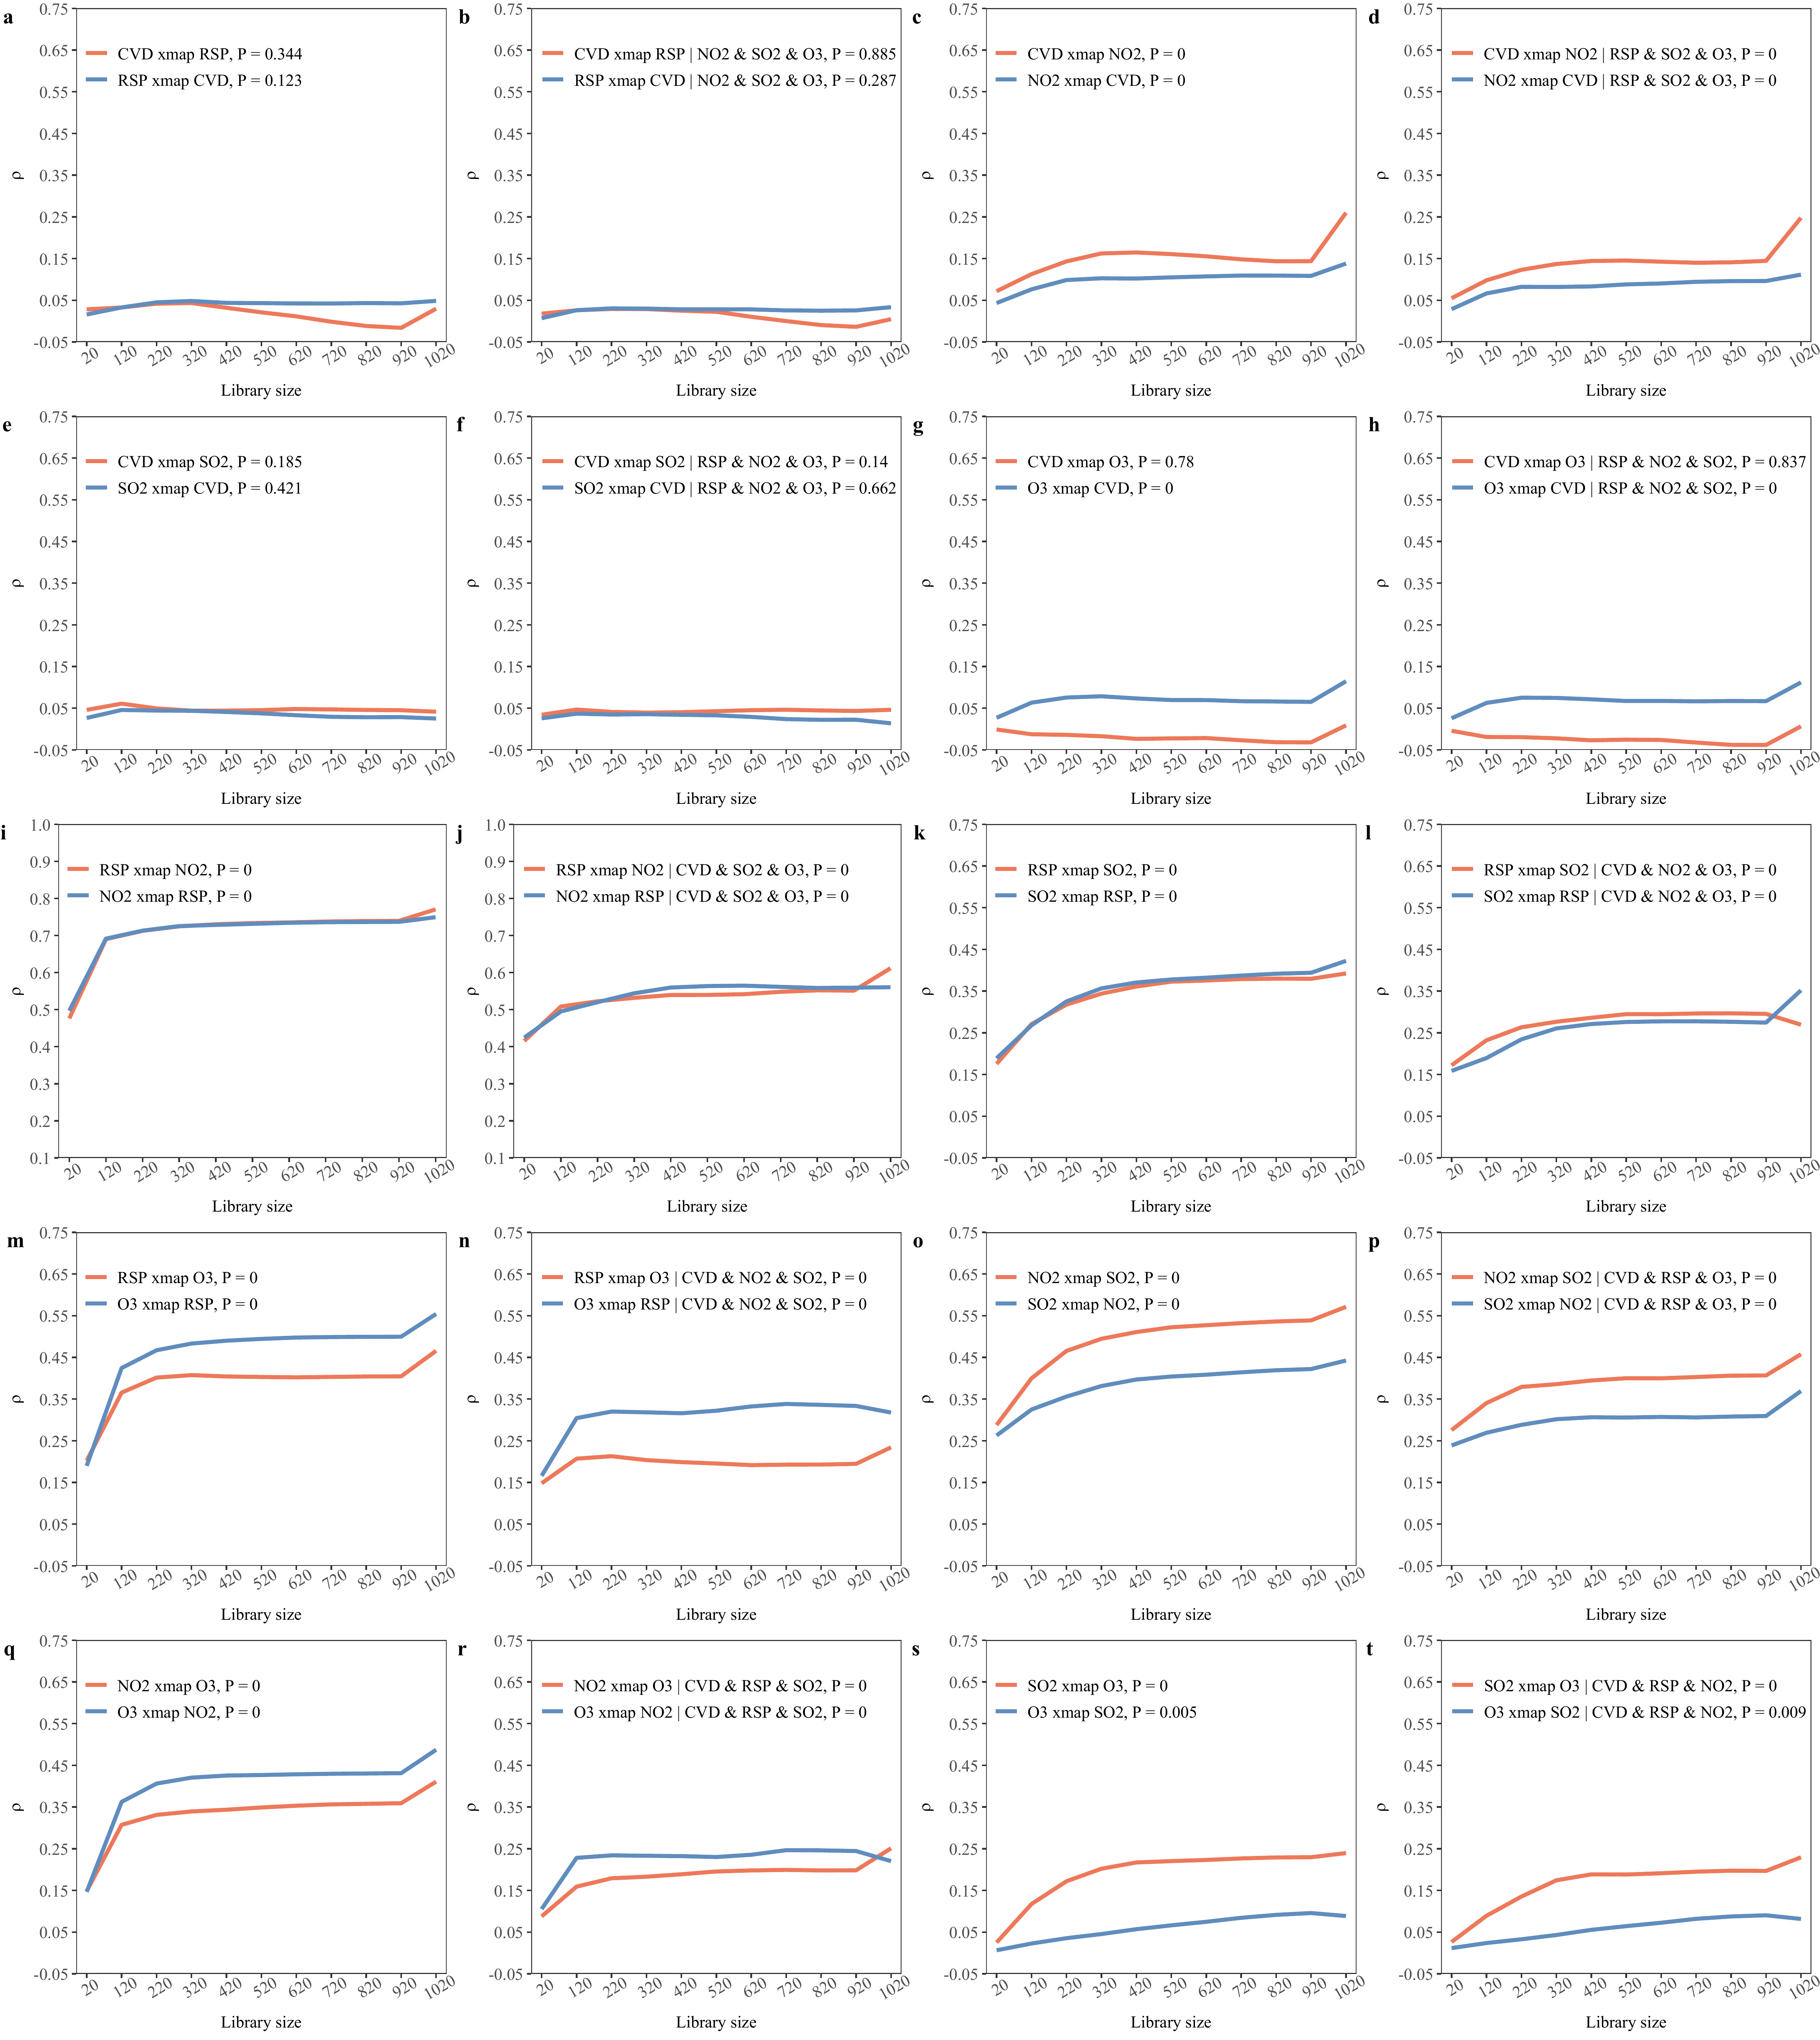
\includegraphics[width=1\textwidth]{./figure/figure_si_1.png}
\caption{Cross mapping skills ($\rho$) between air pollutants and cardiovascular disease incidence, estimated via partial cross mapping across varying library sizes. Here, $x \;\text{xmap}\; y$ denotes the cross mapping from $x$ to $y$, representing the causal direction $y \rightarrow x$, while $x \;\text{xmap}\; y \mid z_1, z_2, \ldots$ denotes the conditional cross-mapping skill of $x$ and $y$ given variables $z_1, z_2, \ldots$.
}
\label{fig_cvds_pcm}
\end{figure}

\begin{figure}[htbp]
\centering
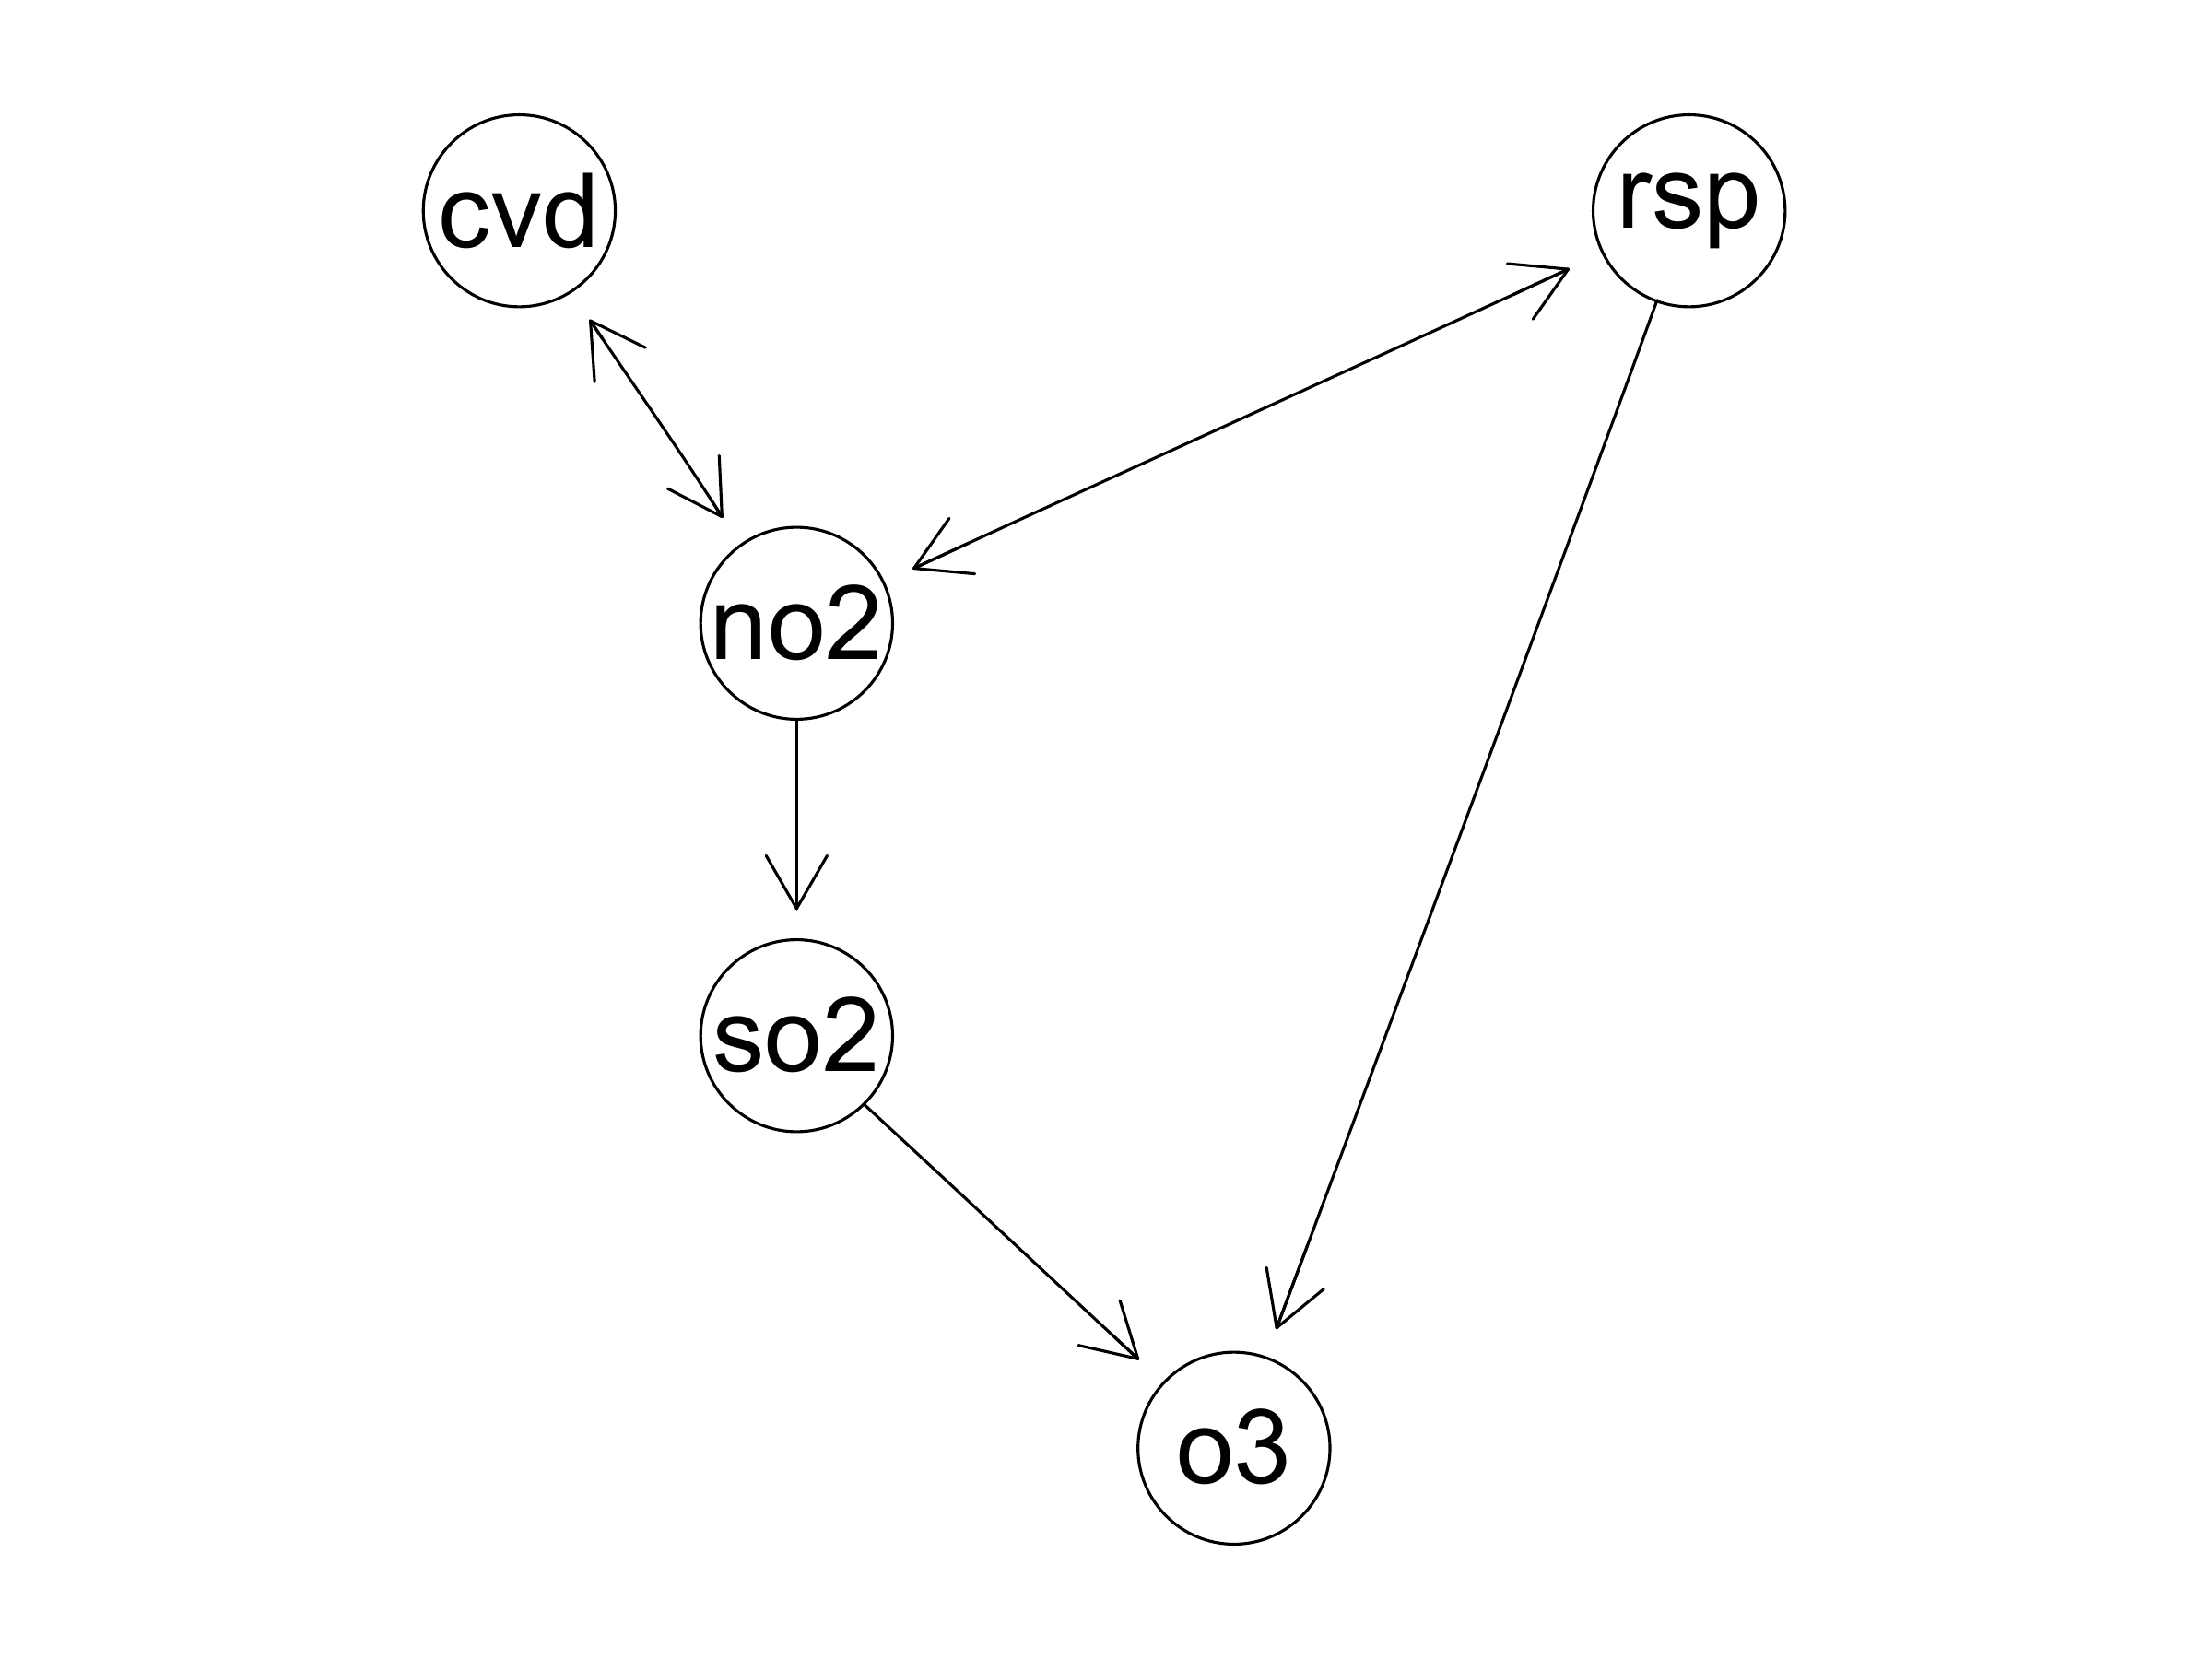
\includegraphics[width=1\textwidth]{./figure/figure_si_2.png}
\caption{Causal netwrok inferred by the PC algorithm for the Hong Kong CVD case study.
}
\label{fig_cvds_pc}
\end{figure}

\begin{figure}[htbp]
\centering

\includegraphics[height=0.75\textwidth]{./figure/figure_si_3.png}
\caption{Results of applying Granger causality to the U.S. carbon emissions case study.
}
\label{fig_carbon_gc}
\end{figure}

\begin{figure}[htbp]
\centering
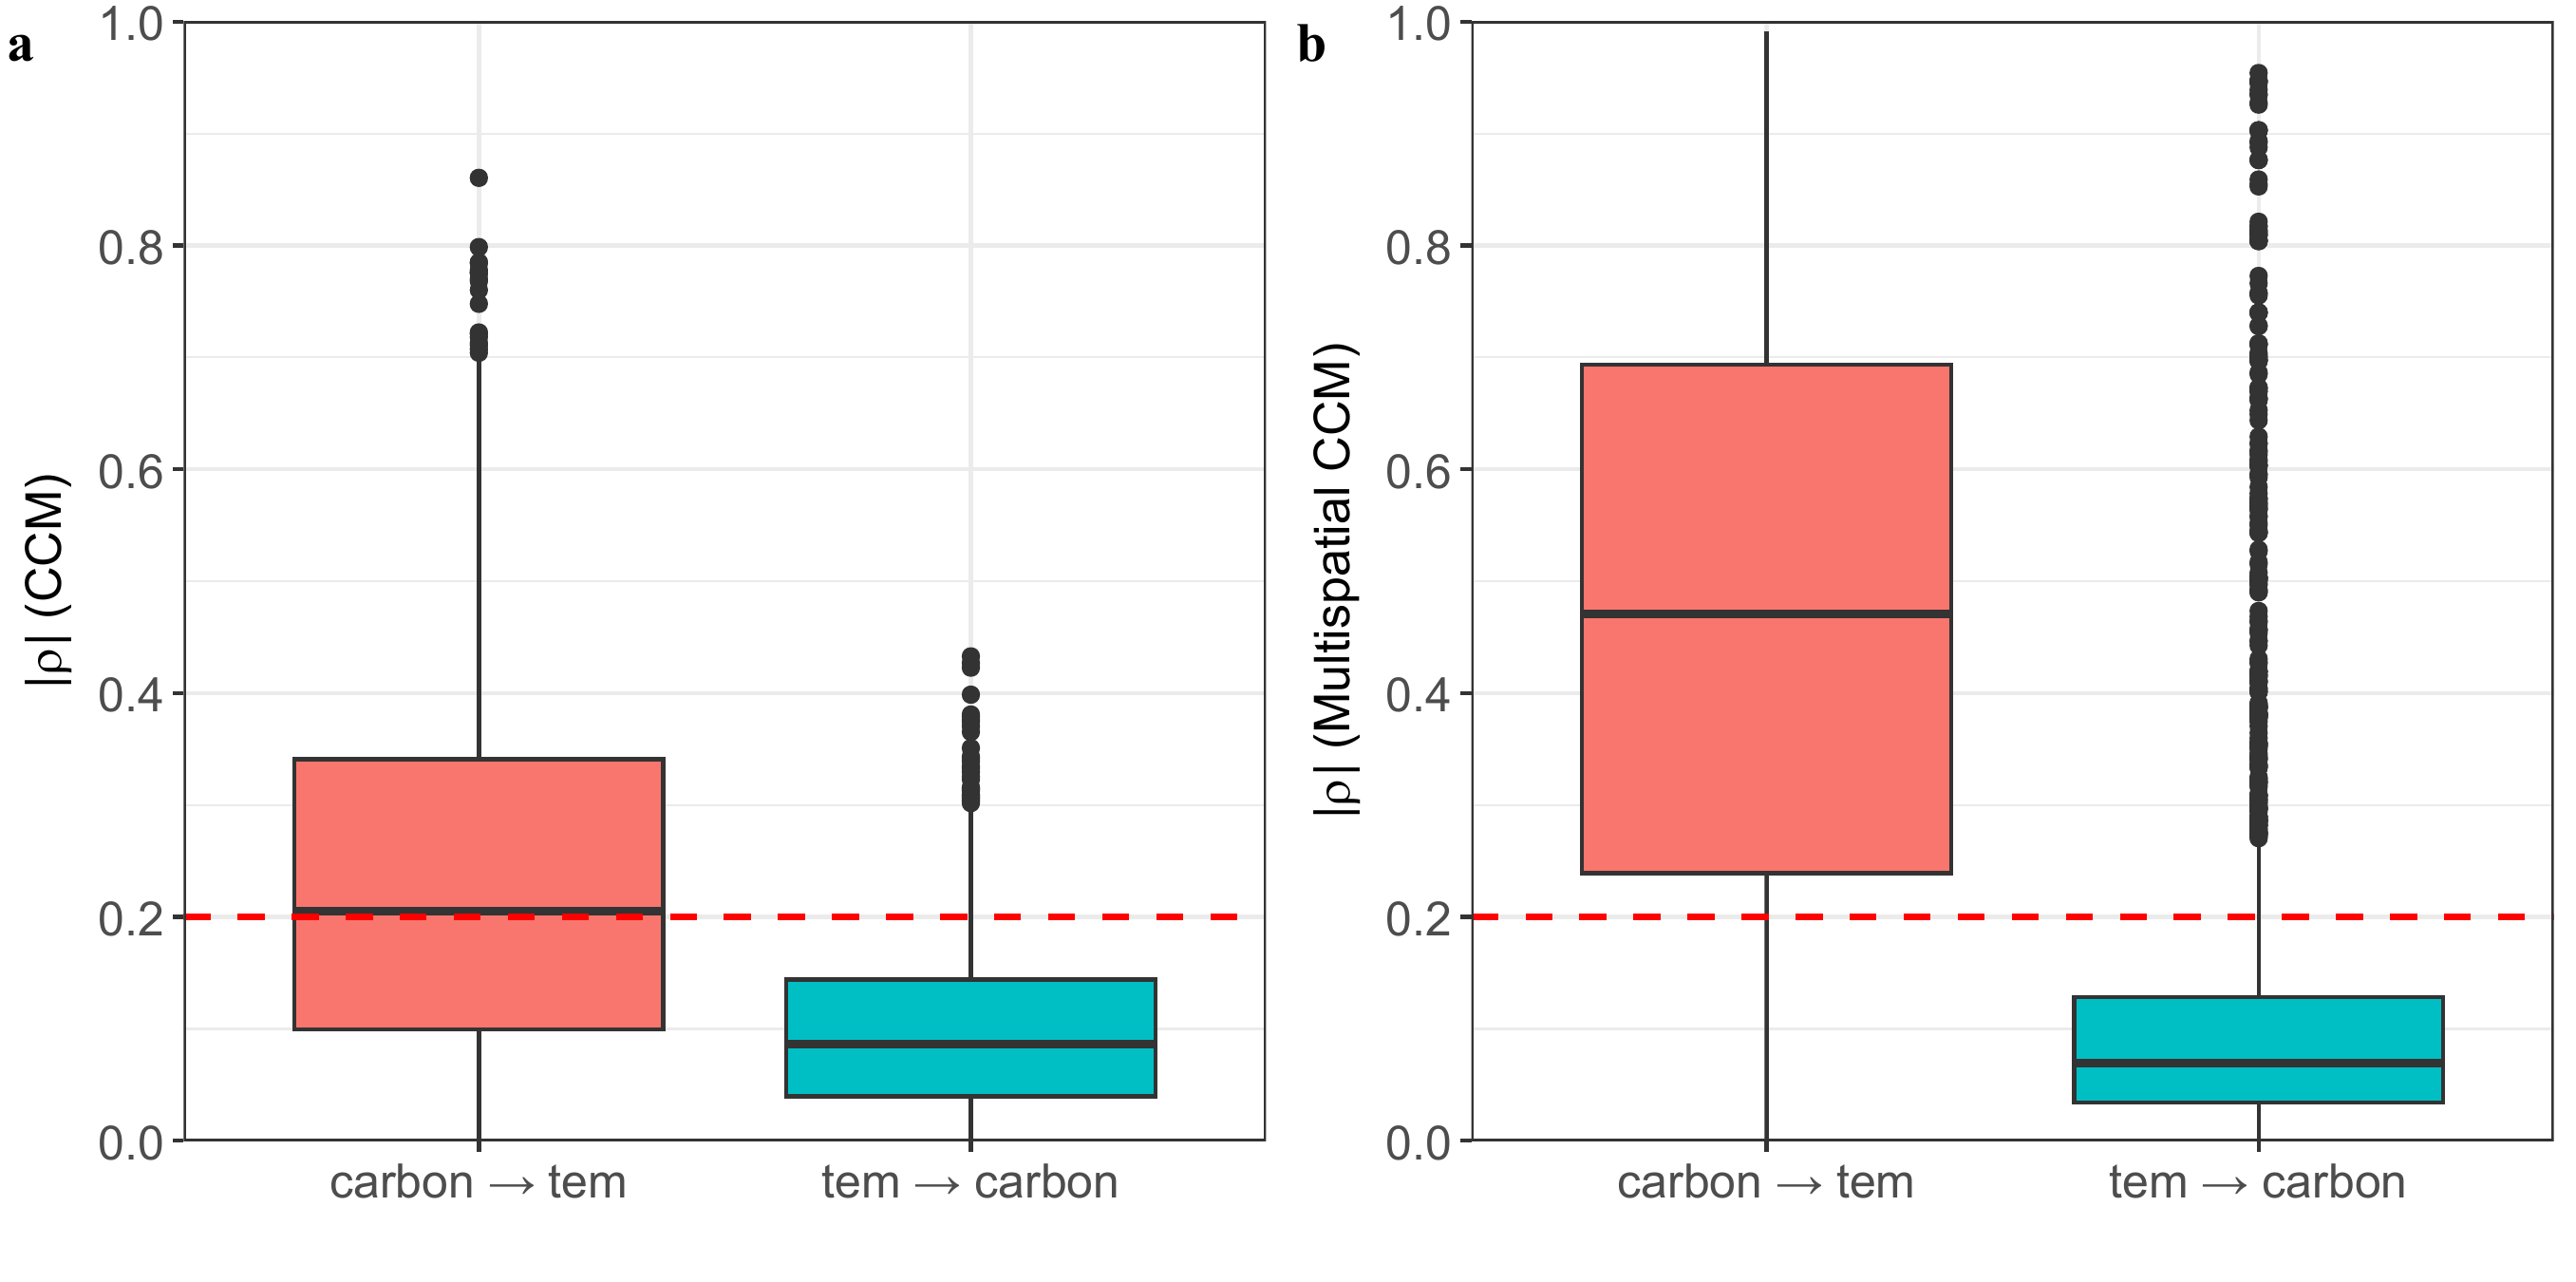
\includegraphics[width=1\textwidth]{./figure/figure_si_4.png}
\caption{Results of applying CCM to the U.S. carbon emissions case study. 
\textbf{a} Results obtained using the original CCM algorithm. 
\textbf{b} Results obtained using the multispatial CCM extension implemented in the \textit{tEDM} package.}
\label{fig_carbon_ccm}
\end{figure}

\begin{figure}[htbp]
\centering

\includegraphics[width=1\textwidth]{./figure/figure_si_5.png}
\caption{Transmission dynamics inferred by the PC algorithm for the Japan COVID-19 case study.
}
\label{fig_covid_pc}
\end{figure}

\end{document}